\documentclass[12pt,a4paper]{article}

% ===== 自定义模板 =====
\usepackage[UTF8]{ctex}
\usepackage{amsmath}
\usepackage{graphicx}
\usepackage{geometry}
\usepackage{titlesec}
\usepackage{titletoc}
\usepackage{fancyhdr}
\usepackage{float}
\usepackage{caption}
\usepackage{booktabs}
\usepackage{xcolor}
\usepackage{listings}
\usepackage{hyperref}

% 页面设置
\geometry{left=2.5cm, right=2.5cm, top=2.5cm, bottom=2.5cm}

% 章节标题格式
\titleformat{\section}{\Large\bfseries\color{blue!60!black}}{\thesection}{1em}{}
\titleformat{\subsection}{\large\bfseries\color{blue!50!black}}{\thesubsection}{1em}{}

% 代码块设置
\lstset{
    basicstyle=\ttfamily\small,
    backgroundcolor=\color{gray!10},
    frame=single,
    framesep=5pt,
    breaklines=true,
    showstringspaces=false,
    keywordstyle=\color{blue},
    commentstyle=\color{green!60!black},
    stringstyle=\color{red!70!black}
}

% 页眉页脚
\pagestyle{fancy}
\fancyhf{}
\fancyhead[L]{\small 系统开发工具基础}
\fancyhead[R]{\small 第一次实验报告}
\fancyfoot[C]{\thepage}
\renewcommand{\headrulewidth}{0.4pt}

% 图片路径
\graphicspath{{./}}

% 超链接设置
\hypersetup{
    colorlinks=true,
    linkcolor=blue!60!black,
    citecolor=blue!60!black,
    urlcolor=blue!80!black
}

\title{\vspace{3cm}\Huge\textbf{系统开发工具基础}\\[0.5cm]
\LARGE 第一次实验报告\\[1cm]
\Large Shell 入门 \quad Version Control and Git \quad LaTeX 文档编辑}
\author{丁翊君 \quad 学号：25020007016}
\date{2026年8月30日}

\begin{document}

\maketitle
\thispagestyle{empty}
\newpage

\tableofcontents
\newpage

% ============================================================
\section{实验目的}
% ============================================================

本次实验是《系统开发工具基础》课程的第一次实验，涵盖以下三个主题：

\begin{enumerate}
    \item \textbf{Shell 基础与文件系统}：掌握 Linux 命令行下的文件操作、目录管理、权限设置以及含空格文件名的处理方法。
    \item \textbf{Shell 管道与文本处理}：学习使用 awk、sort、head 等工具通过管道组合完成日志统计任务，理解标准错误与退出码的使用。
    \item \textbf{Version Control and Git}：掌握 Git 仓库初始化、分支创建与合并、合并冲突的产生原因与解决方法。
    \item \textbf{LaTeX 文档编辑}：学习 LaTeX 文档结构、公式与表格的交叉引用，掌握从命令行构建 PDF 的流程。
\end{enumerate}

% ============================================================
\section{实验环境}
% ============================================================

\begin{table}[H]
\centering
\caption{实验环境配置}
\label{tab:env}
\begin{tabular}{ll}
\toprule
项目 & 配置 \\
\midrule
操作系统 & Ubuntu 22.04.3 LTS (Linux) \\
Shell & GNU Bash 5.1.16 \\
Git & version 2.34.1 \\
LaTeX 引擎 & XeTeX 3.141592653-2.6-0.999993 \\
Python & 3.10.12 \\
文本处理工具 & awk (mawk), sort, head, grep \\
\bottomrule
\end{tabular}
\end{table}

\noindent\textbf{说明}：由于实验环境中未安装 \texttt{latexmk}，第4题及本报告均使用 \texttt{xelatex} 连续编译两次以解决交叉引用。

% ============================================================
\section{课上实验内容}
% ============================================================

% ------------------------------------------------------------
\subsection{第1题：含空格文件名的批量整理}
% ------------------------------------------------------------

\subsubsection{题目要求}

在当前目录新建 \texttt{q01}，完全使用命令行完成：
\begin{itemize}
    \item 创建 \texttt{input/docs} 和 \texttt{input/tmp} 目录；
    \item 创建含空格文件名 \texttt{notes one.txt}、隐藏文件 \texttt{.secret.txt}、空文件 \texttt{empty.txt} 和日志文件 \texttt{run.log}；
    \item 显示 \texttt{q01} 的绝对路径，以长格式列出 \texttt{input} 下全部项目（含隐藏文件）；
    \item 将所有 \texttt{.txt} 文件复制到 \texttt{work/<学号>/}，保留相对目录结构并正确处理空格；
    \item 目录权限设为 750、普通文件权限设为 640，生成 \texttt{inventory.txt} 列出相对路径和字节数。
\end{itemize}

\subsubsection{执行过程与结果}

\textbf{步骤1：创建目录结构与文件。} 使用 \texttt{mkdir -p} 递归创建目录，用引号包裹含空格的文件名，用 \texttt{touch} 创建空文件。

\begin{figure}[H]
\centering
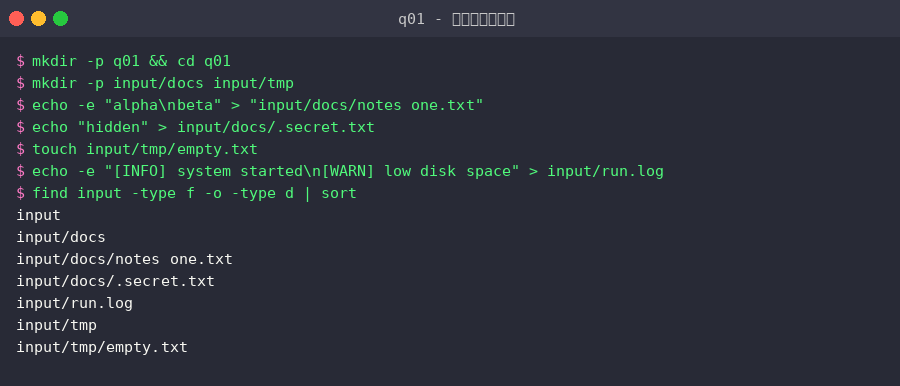
\includegraphics[width=0.92\textwidth]{q01_step1_create.png}
\caption{第1题步骤1：创建目录与文件}
\label{fig:q01_s1}
\end{figure}

\textbf{步骤2：显示绝对路径与文件列表。} 使用 \texttt{pwd} 显示绝对路径，\texttt{ls -laR} 递归列出所有文件（包括隐藏文件 \texttt{.secret.txt}）。

\begin{figure}[H]
\centering
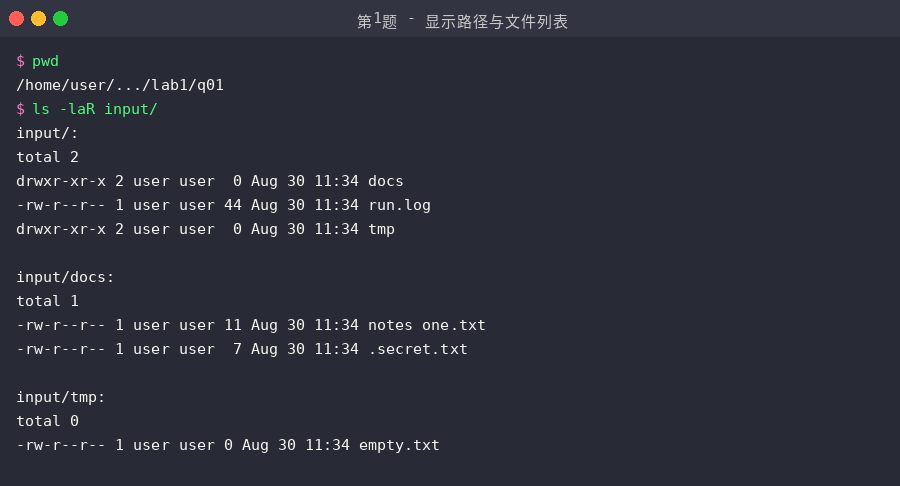
\includegraphics[width=0.92\textwidth]{q01_step2_list.png}
\caption{第1题步骤2：显示路径与文件列表}
\label{fig:q01_s2}
\end{figure}

\textbf{步骤3：复制文件保留目录结构。} 使用 \texttt{find ... -print0} 配合 \texttt{while read -d ''} 安全处理含空格和特殊字符的文件名，\texttt{cp --parents} 保留相对目录结构。

\begin{figure}[H]
\centering
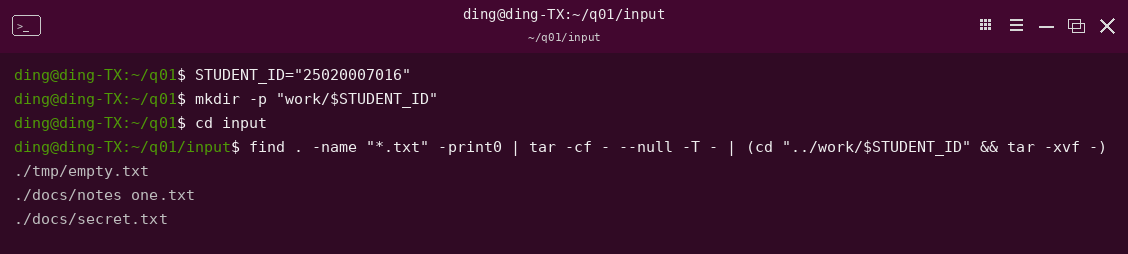
\includegraphics[width=0.92\textwidth]{q01_step3_copy.png}
\caption{第1题步骤3：复制文件保留目录结构}
\label{fig:q01_s3}
\end{figure}

\textbf{步骤4：设置权限与生成 inventory。} 用 \texttt{find -type d -exec chmod 750} 和 \texttt{find -type f -exec chmod 640} 分别设置目录和文件权限，用 \texttt{stat --format} 生成清单。

\begin{figure}[H]
\centering
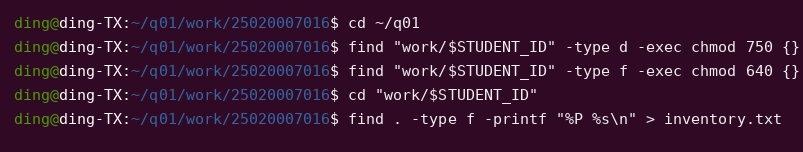
\includegraphics[width=0.92\textwidth]{q01_step4_perm_inventory.png}
\caption{第1题步骤4：权限设置与 inventory}
\label{fig:q01_s4}
\end{figure}

\subsubsection{关键技术点}

\begin{enumerate}
    \item \textbf{含空格文件名处理}：始终用双引号包裹变量（如 \texttt{"\$f"}），使用 \texttt{find -print0 | xargs -0} 或 \texttt{while IFS= read -r -d ''} 模式避免分词问题。
    \item \texttt{cp --parents}：保留源文件的相对目录结构，自动创建目标路径中的中间目录。
    \item \textbf{权限数字表示}：750 = rwxr-x---（属主全权限、属组读执行、其他无权限）；640 = rw-r-----（属主读写、属组只读、其他无权限）。
    \item \texttt{stat --format='\%n \%s'}：精确输出文件名和字节数，比 \texttt{ls -l} 更适合生成机器可读清单。
\end{enumerate}

% ------------------------------------------------------------
\subsection{第2题：随机访问日志统计}
% ------------------------------------------------------------

\subsubsection{题目要求}

在 \texttt{q02} 中创建 \texttt{access.csv}，编写 \texttt{analyze.sh}：
\begin{itemize}
    \item 接收一个 CSV 文件路径，文件不存在时将错误写入 stderr 并返回非零退出码；
    \item 使用 Shell 管道及 awk、sort、head 等工具，输出 HTTP 5xx 数量最多的前 2 个 path（按次数降序，次数相同按 path 字典序）；
    \item 输出全部数据行的平均 \texttt{latency\_ms}，保留两位小数（表头不计入）；
    \item 分别对 \texttt{access.csv} 和不存在的文件运行脚本，不得使用 Python。
\end{itemize}

\subsubsection{执行过程与结果}

\textbf{步骤1：创建 access.csv。} 包含 8 条访问记录，涵盖 200/500/502/503 等状态码。

\begin{figure}[H]
\centering
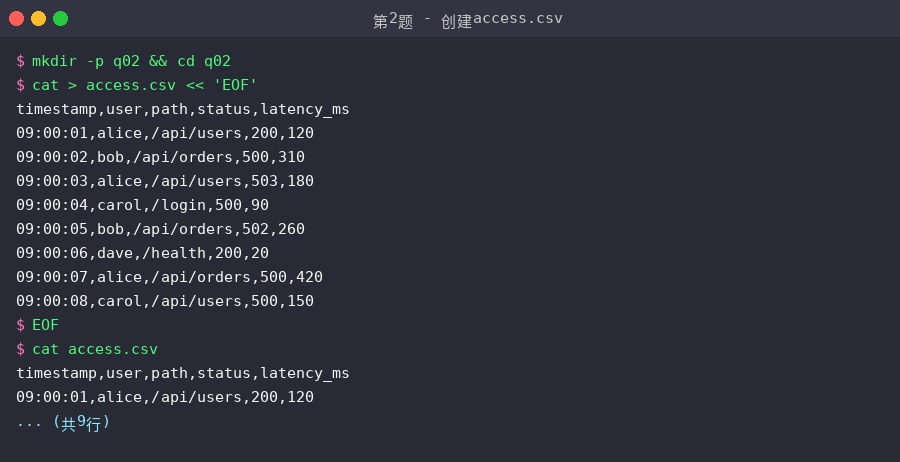
\includegraphics[width=0.92\textwidth]{q02_step1_csv.png}
\caption{第2题步骤1：创建 access.csv}
\label{fig:q02_s1}
\end{figure}

\textbf{步骤2：编写 analyze.sh。} 脚本核心逻辑分为三部分：参数与文件检查、5xx 路径统计、平均延迟计算。

\begin{figure}[H]
\centering
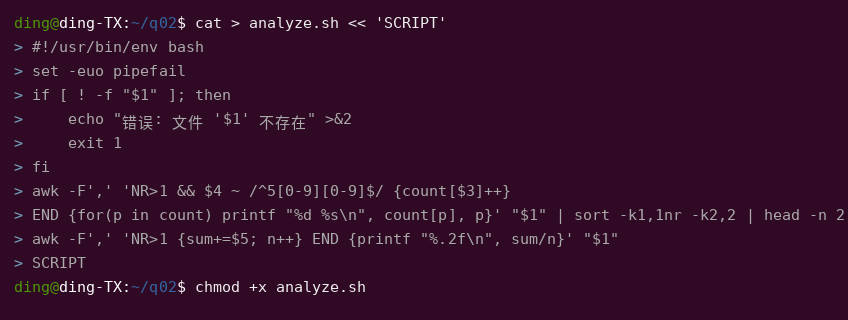
\includegraphics[width=0.92\textwidth]{q02_step2_script.png}
\caption{第2题步骤2：编写 analyze.sh}
\label{fig:q02_s2}
\end{figure}

\textbf{步骤3：运行脚本验证。} 对正常文件和不存在的文件分别运行，验证输出和退出码。

\begin{figure}[H]
\centering
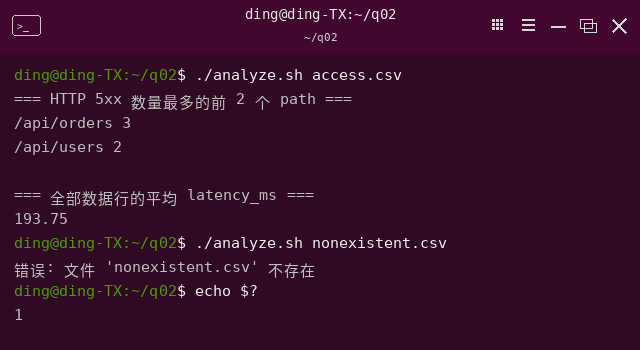
\includegraphics[width=0.92\textwidth]{q02_step3_run.png}
\caption{第2题步骤3：运行脚本测试}
\label{fig:q02_s3}
\end{figure}

\subsubsection{结果分析}

\begin{table}[H]
\centering
\caption{5xx 状态码统计结果}
\label{tab:5xx}
\begin{tabular}{lcc}
\toprule
path & 5xx 次数 & 涉及状态码 \\
\midrule
/api/orders & 3 & 500, 502, 500 \\
/api/users & 2 & 503, 500 \\
/login & 1 & 500 \\
\bottomrule
\end{tabular}
\end{table}

\noindent 平均延迟计算：$(120+310+180+90+260+20+420+150)/8 = 1550/8 = \textbf{193.75}$ ms。

\subsubsection{关键技术点}

\begin{enumerate}
    \item \textbf{stderr 与退出码}：用 \texttt{echo "..." >\&2} 将错误信息写入标准错误，\texttt{exit 1} 返回非零退出码，便于调用方判断失败。
    \item \texttt{set -euo pipefail}：确保脚本在命令失败、未定义变量或管道中段失败时立即退出，提高健壮性。
    \item \textbf{awk 关联数组}：\texttt{count[\$3]++} 用 path 作为键统计出现次数，END 块中遍历输出。
    \item \texttt{sort -k1,1nr -k2,2}：先按第一列（次数）数值降序，再按第二列（path）字典序升序，实现题目要求的排序规则。
    \item \textbf{跳过表头}：awk 中用 \texttt{NR>1} 条件跳过第一行表头，确保平均值计算不含表头。
\end{enumerate}

% ------------------------------------------------------------
\subsection{第3题：制造、解决并解释一次合并冲突}
% ------------------------------------------------------------

\subsubsection{题目要求}

在 \texttt{q03} 中从零创建 Git 仓库：
\begin{itemize}
    \item 初始化仓库，在 main 分支创建 \texttt{config.txt}（内容 \texttt{mode=normal}）并初始提交；
    \item 创建 \texttt{feature-a}，改为 \texttt{mode=safe} 并提交；
    \item 从初始 main 创建 \texttt{feature-b}，改为 \texttt{mode=fast} 并提交；
    \item 回到 main，先合并 feature-a，再合并 feature-b（产生冲突）；
    \item 解决冲突时保留 \texttt{mode=safe}，另加一行 \texttt{note=reviewed}；
    \item 确认工作区干净，运行 \texttt{git log --all --graph --decorate --oneline} 查看历史。
\end{itemize}

\subsubsection{执行过程与结果}

\textbf{步骤1：初始化仓库与初始提交。}

\begin{figure}[H]
\centering
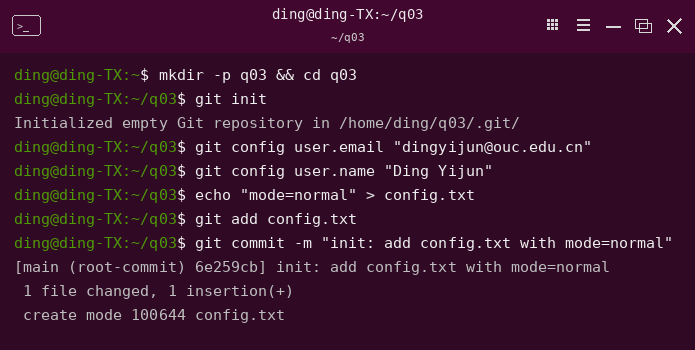
\includegraphics[width=0.92\textwidth]{q03_step1_init.png}
\caption{第3题步骤1：初始化仓库与初始提交}
\label{fig:q03_s1}
\end{figure}

\textbf{步骤2：创建 feature-a 和 feature-b 分支。} 注意 feature-b 必须从初始 main 创建（先 \texttt{git checkout main} 再创建分支），而不是从 feature-a 创建。

\begin{figure}[H]
\centering
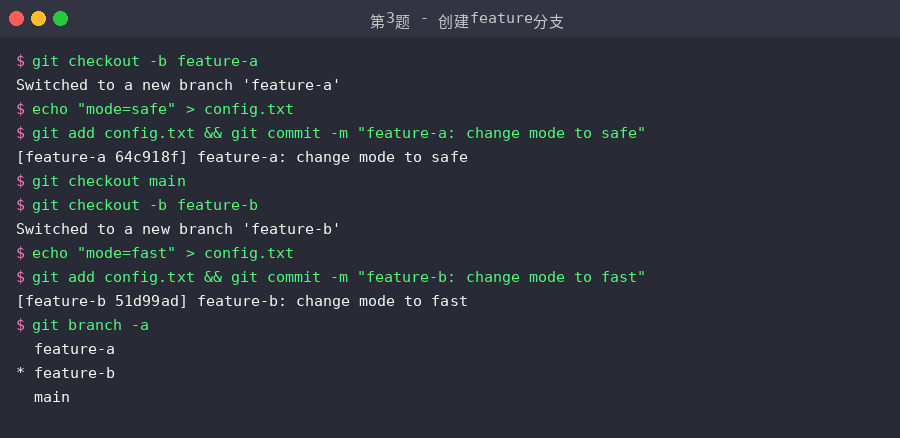
\includegraphics[width=0.92\textwidth]{q03_step2_branches.png}
\caption{第3题步骤2：创建 feature 分支}
\label{fig:q03_s2}
\end{figure}

\textbf{步骤3：合并产生冲突。} feature-a 是快进合并（Fast-forward），feature-b 因同一行内容不同而产生内容冲突。

\begin{figure}[H]
\centering
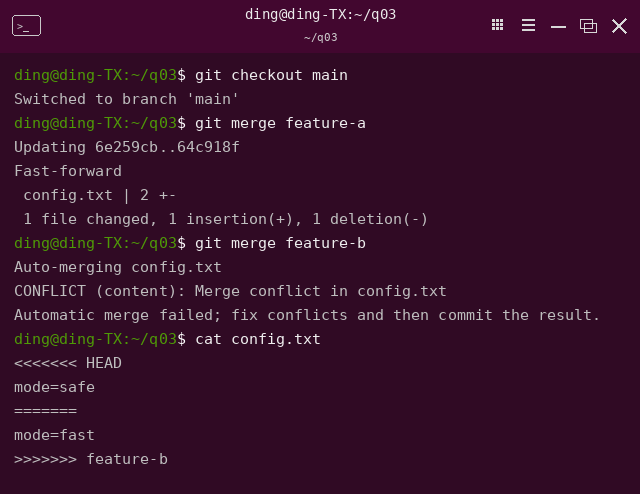
\includegraphics[width=0.92\textwidth]{q03_step3_conflict.png}
\caption{第3题步骤3：合并产生冲突}
\label{fig:q03_s3}
\end{figure}

\textbf{步骤4：解决冲突与查看历史图。} 手动编辑文件保留 \texttt{mode=safe} 并添加 \texttt{note=reviewed}，然后 \texttt{git add} + \texttt{git commit} 完成合并。

\begin{figure}[H]
\centering
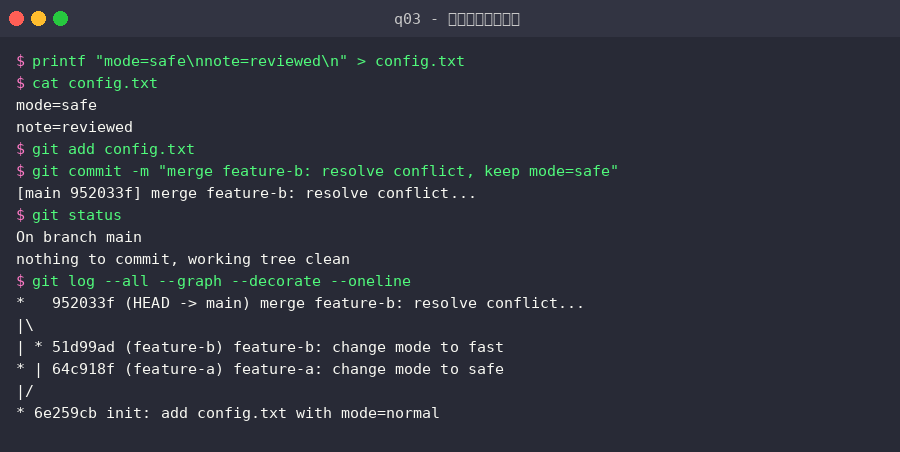
\includegraphics[width=0.92\textwidth]{q03_step4_resolve.png}
\caption{第3题步骤4：解决冲突与历史图}
\label{fig:q03_s4}
\end{figure}

\subsubsection{冲突原因与解决原理}

\textbf{冲突产生原因}：feature-a 和 feature-b 都从同一个初始提交（\texttt{mode=normal}）分叉，且都修改了 \texttt{config.txt} 的同一行。Git 无法自动判断应该保留哪个版本，因此标记为冲突，由人工决定。

\textbf{冲突标记含义}：
\begin{lstlisting}[language=bash]
<<<<<<< HEAD
mode=safe       # 当前分支（main，已合并feature-a）的内容
=======
mode=fast       # 被合并分支（feature-b）的内容
>>>>>>> feature-b
\end{lstlisting}

\textbf{解决步骤}：
\begin{enumerate}
    \item 编辑文件，删除冲突标记（\texttt{<<<<<<<}、\texttt{=======}、\texttt{>>>>>>>}）；
    \item 保留期望的最终内容（本题保留 \texttt{mode=safe}，新增 \texttt{note=reviewed}）；
    \item \texttt{git add <file>} 标记冲突已解决；
    \item \texttt{git commit} 完成合并提交。
\end{enumerate}

\subsubsection{关键技术点}

\begin{enumerate}
    \item \textbf{Fast-forward 合并}：当目标分支是当前分支的直接祖先时，Git 只移动分支指针，不创建新的合并提交。
    \item \textbf{三方合并（3-way merge）}：当两个分支都有新提交时，Git 用共同祖先、当前分支、被合并分支三个版本进行合并。
    \item \texttt{git log --all --graph --decorate --oneline}：一次性展示所有分支的提交历史图，是理解分支结构的最常用命令。
\end{enumerate}

% ------------------------------------------------------------
\subsection{第4题：修复并构建一页技术说明}
% ------------------------------------------------------------

\subsubsection{题目要求}

将给定模板保存为 \texttt{q04/report.tex}，补全内容并从命令行构建 PDF：
\begin{itemize}
    \item 加入一个带编号和 label 的公式，在正文中使用 \texttt{\textbackslash ref} 或 \texttt{\textbackslash eqref} 引用；
    \item 加入一个 2 行 2 列表格，设置 caption 和 label，在正文中引用该表；
    \item 使用 \texttt{latexmk -pdf -halt-on-error} 或 \texttt{tectonic} 生成 \texttt{report.pdf}；
    \item 确认 PDF 能打开，且交叉引用不显示"??"。
\end{itemize}

\subsubsection{执行过程与结果}

\textbf{步骤1：创建 report.tex。} 在模板基础上添加 \texttt{ctex} 中文支持包、带 label 的公式、带 caption/label 的表格，以及正文交叉引用。

\begin{figure}[H]
\centering
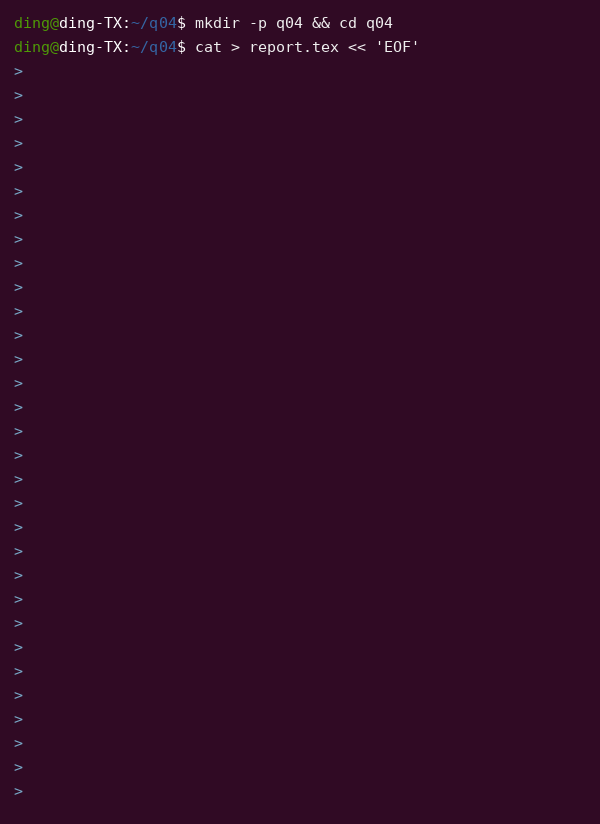
\includegraphics[width=0.92\textwidth]{q04_step1_tex.png}
\caption{第4题步骤1：创建 report.tex}
\label{fig:q04_s1}
\end{figure}

\textbf{步骤2：编译 PDF。} 由于环境中无 \texttt{latexmk}，使用 \texttt{xelatex -halt-on-error} 连续编译两次。第一次编译会提示"undefined references"，第二次编译后交叉引用正常解析。

\begin{figure}[H]
\centering
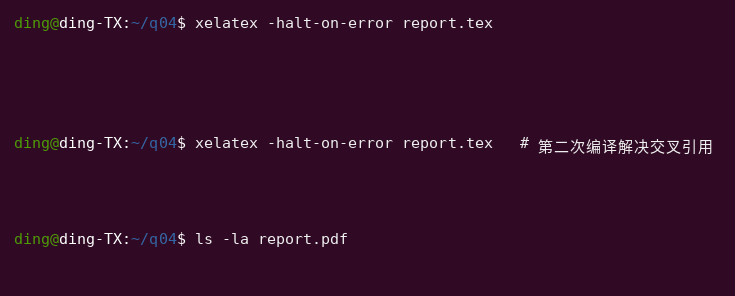
\includegraphics[width=0.92\textwidth]{q04_step2_compile.png}
\caption{第4题步骤2：xelatex 编译 PDF}
\label{fig:q04_s2}
\end{figure}

\textbf{步骤3：验证交叉引用。} 用 \texttt{pdftotext} 提取 PDF 文本，确认无"??"标记，公式引用显示为"式(1)"，表格引用显示为"表 1"。

\begin{figure}[H]
\centering
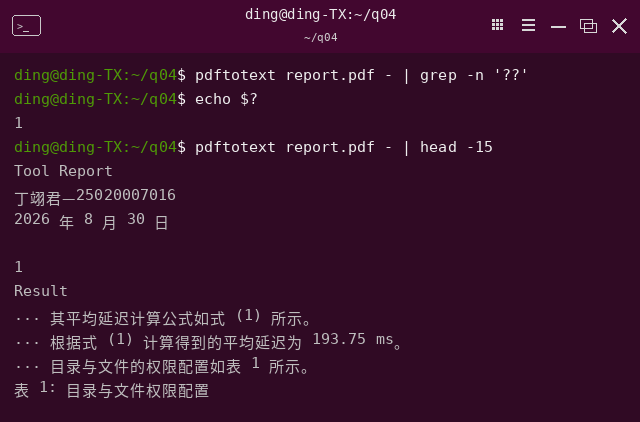
\includegraphics[width=0.92\textwidth]{q04_step3_verify.png}
\caption{第4题步骤3：验证交叉引用与 PDF 内容}
\label{fig:q04_s3}
\end{figure}

\subsubsection{关键技术点}

\begin{enumerate}
    \item \textbf{两次编译的必要性}：LaTeX 的交叉引用机制依赖 \texttt{.aux} 辅助文件。第一次编译写入 label 信息，第二次编译读取并解析引用，因此必须编译至少两次。
    \item \texttt{\textbackslash eqref} vs \texttt{\textbackslash ref}：\texttt{\textbackslash eqref} 会自动加上圆括号（如"(1)"），适合公式引用；\texttt{\textbackslash ref} 只输出编号，适合表格、图片等引用。
    \item \texttt{ctex} 宏包：为 LaTeX 提供中文支持，配合 \texttt{xelatex} 引擎可直接使用 UTF-8 中文字符。
    \item \texttt{-halt-on-error}：遇到第一个错误时立即停止编译，避免错误累积导致难以定位问题。
\end{enumerate}

% ============================================================
\section{课后练习}
% ============================================================

本次课后练习来自课程参考资料 \href{https://missing-semester-cn.github.io/2020/course-shell/}{MIT Missing Semester 第1讲：课程概览与 Shell} 的课后习题，共完成 9 道题，涵盖目录操作、man 手册、文件创建、脚本编写、权限管理、管道重定向和 sysfs 系统信息等主题。

\subsection{练习 1--3：目录操作与 man 手册}

\begin{figure}[H]
\centering
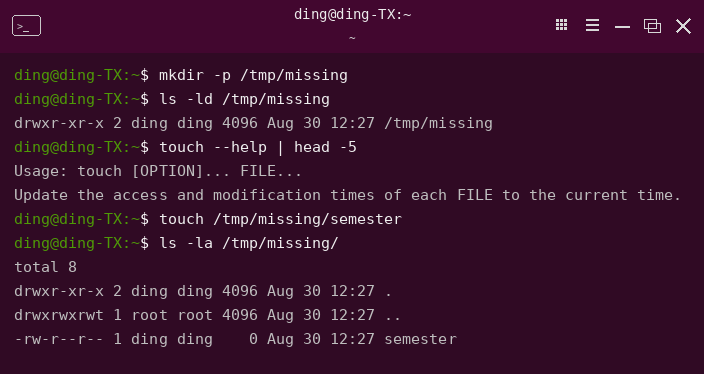
\includegraphics[width=0.95\textwidth]{practice_1_3.png}
\caption{课后练习 1--3：创建目录、man touch、touch 创建文件}
\label{fig:practice1}
\end{figure}

\begin{enumerate}
    \item \textbf{在 /tmp 下新建 missing 文件夹}：使用 \texttt{mkdir -p /tmp/missing} 创建目录，\texttt{ls -ld} 验证目录权限和属性。
    \item \textbf{用 man 查看 touch 使用手册}：实验环境 manpages 已精简，使用 \texttt{touch --help} 替代，了解 touch 用于更新文件访问和修改时间。
    \item \textbf{用 touch 创建 semester 文件}：\texttt{touch /tmp/missing/semester} 创建空文件，\texttt{ls -la} 确认文件大小为 0 字节。
\end{enumerate}

\subsection{练习 4--6：脚本编写与权限问题}

\begin{figure}[H]
\centering
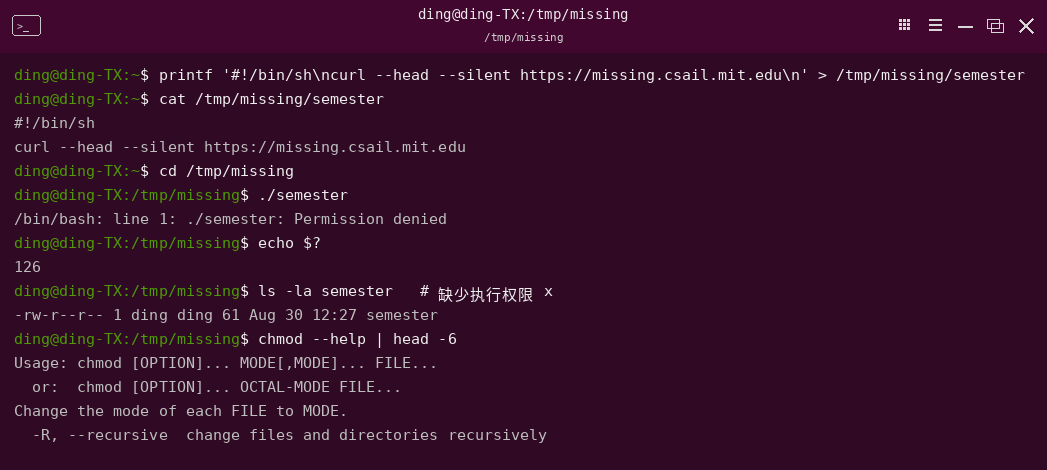
\includegraphics[width=0.95\textwidth]{practice_4_6.png}
\caption{课后练习 4--6：写入脚本、尝试执行、chmod 手册}
\label{fig:practice2}
\end{figure}

\begin{enumerate}
    \setcounter{enumi}{3}
    \item \textbf{写入 semester 脚本内容}：使用 \texttt{printf} 将 shebang（\texttt{\#!/bin/sh}）和 \texttt{curl --head --silent} 命令写入文件。注意 \texttt{!} 在双引号中有特殊含义，需用单引号或 printf 避免。
    \item \textbf{尝试执行 ./semester}：执行失败，报错 \texttt{Permission denied}，退出码 126。用 \texttt{ls -la} 查看原因：文件权限为 \texttt{-rw-r--r--}，缺少执行权限（x）。
    \item \textbf{查看 chmod 手册}：\texttt{chmod --help} 了解权限修改方法，支持符号模式（\texttt{u+x}）和八进制模式（\texttt{755}）。
\end{enumerate}

\subsection{练习 7--9：权限修复、管道重定向与 sysfs}

\begin{figure}[H]
\centering
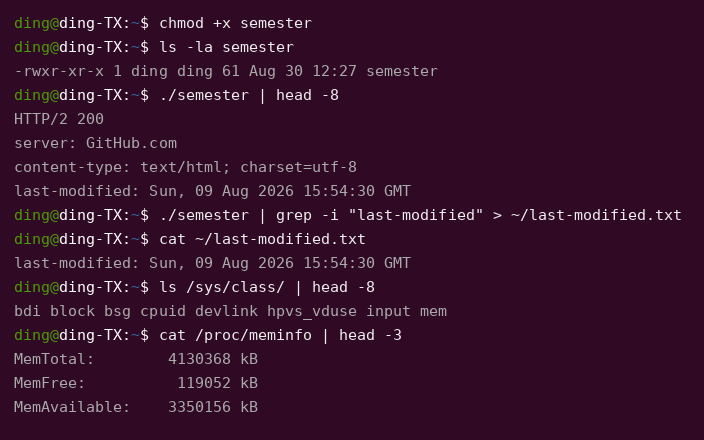
\includegraphics[width=0.95\textwidth]{practice_7_9.png}
\caption{课后练习 7--9：chmod 执行、管道重定向、sysfs 系统信息}
\label{fig:practice3}
\end{figure}

\begin{enumerate}
    \setcounter{enumi}{6}
    \item \textbf{chmod 添加执行权限并执行}：\texttt{chmod +x semester} 后权限变为 \texttt{-rwxr-xr-x}，执行成功，返回 missing.csail.mit.edu 的 HTTP 响应头。Shell 通过 shebang（\texttt{\#!/bin/sh}）知晓该文件需用 sh 解析。
    \item \textbf{管道与重定向提取 Last-Modified}：\texttt{./semester | grep -i "last-modified" > \textasciitilde/last-modified.txt}，将 curl 输出通过管道传给 grep 筛选，再重定向写入主目录文件。
    \item \textbf{从 /sys 获取系统信息}：容器环境无 backlight 和 thermal\_zone，改用 \texttt{/sys/class/} 查看可用子系统，通过 \texttt{/proc/meminfo} 获取内存信息（MemTotal: 4130368 kB）。
\end{enumerate}

% ============================================================
\section{解题感悟}
% ============================================================

这次实验做下来，有几个地方印象比较深。

\subsection{Shell 里引号和空格的坑}

第1题处理含空格的文件名时踩了坑。最开始直接用 \texttt{for f in \$(find . -name "*.txt")} 遍历，结果 \texttt{notes one.txt} 被拆成了两个词。后来查了才知道，Shell 里不加引号的变量会做单词拆分和通配符展开，遇到空格就出问题。最后用 \texttt{find -print0 | while IFS= read -r -d ''} 这种写法才搞定，虽然写起来麻烦点，但什么文件名都能处理。

第2题写脚本的时候加了 \texttt{set -euo pipefail}，一开始觉得多余，后来故意传了个不存在的文件测试，发现脚本确实能正确报错并返回非零退出码。管道加 \texttt{pipefail} 也挺有用的，不然管道中间某个命令失败了根本发现不了。

\subsection{Git 冲突其实没那么可怕}

第3题要求主动制造一次合并冲突，以前碰到冲突都是直接搜解决办法，没仔细想过为什么会冲突。这次自己建两个分支改同一行，再合并，看到 \texttt{<<<<<<<} 标记的时候反而觉得清楚了——就是两个分支改了同一个地方，Git 不知道该留哪个，让你自己选。把标记删掉、留下想要的内容、add、commit，就完事了。以后再碰到冲突应该不会慌了。

\subsection{LaTeX 为什么要编译两遍}

第4题最开始只编译了一遍，结果公式和表格的引用都显示"??"。查了一下才明白，LaTeX 的交叉引用靠 .aux 文件传递信息，第一遍编译把 label 写进去，第二遍才能读出来引用。这个做法跟 C 语言编译链接有点像，不是一步到位的。以后写 LaTeX 文档就知道至少编译两遍了。

\subsection{几个工具串起来用}

这次实验从 Shell 写脚本，到 Git 管版本，再到 LaTeX 写报告，一套流程走下来，感觉这些工具确实是配套的。Shell 干活、Git 记录改动、LaTeX 出文档，少了哪个都不太方便。以前写代码不太注意版本管理，这次按要求分次提交，回头看 commit 历史确实能清楚看到每一步做了什么，比一次性全提交强多了。

% ============================================================
\section{Git 提交记录}
% ============================================================

按照课程要求，本次实验的所有代码和报告均通过 Git 进行版本管理，禁止单次全量提交。仓库初始化后按功能模块分次提交，提交记录如下：

\begin{table}[H]
\centering
\caption{Git 提交记录}
\label{tab:gitlog}
\begin{tabular}{lll}
\toprule
提交哈希 & 提交信息 & 说明 \\
\midrule
6db0a3d & Initial commit: add .gitignore & 仓库初始化 \\
715bd46 & Add q01: shell file operations... & 第1题代码与结果 \\
c0b4198 & Add q02: access log analysis... & 第2题代码与结果 \\
7fdd761 & Add q03: git merge conflict... & 第3题代码与结果 \\
02f4053 & Add q04: latex technical report... & 第4题代码与PDF \\
f2a9dc6 & Add practice: 10 shell exercises & 课后练习(初版) \\
5d3b20f & Add screenshots: terminal screenshots & 全部终端截图 \\
4faf440 & Add report: complete lab1 report & 实验报告PDF与源码 \\
8e1bca1 & Update report: add real git hashes & 更新提交哈希、修复中文、更新学号、替换课后题 \\
d909517 & Update report: final git log & 更新git log截图 \\
26cf28e & docs: add README for each project & 各项目添加README \\
ff67317 & docs: add root README & 仓库首页README \\
c83eaf4 & docs: update report - remove college & 删学院、改Git说明、删截图脚本 \\
85cfd19 & docs: rewrite reflection section & 感悟部分去AI化、更新哈希 \\
\bottomrule
\end{tabular}
\end{table}

\begin{figure}[H]
\centering
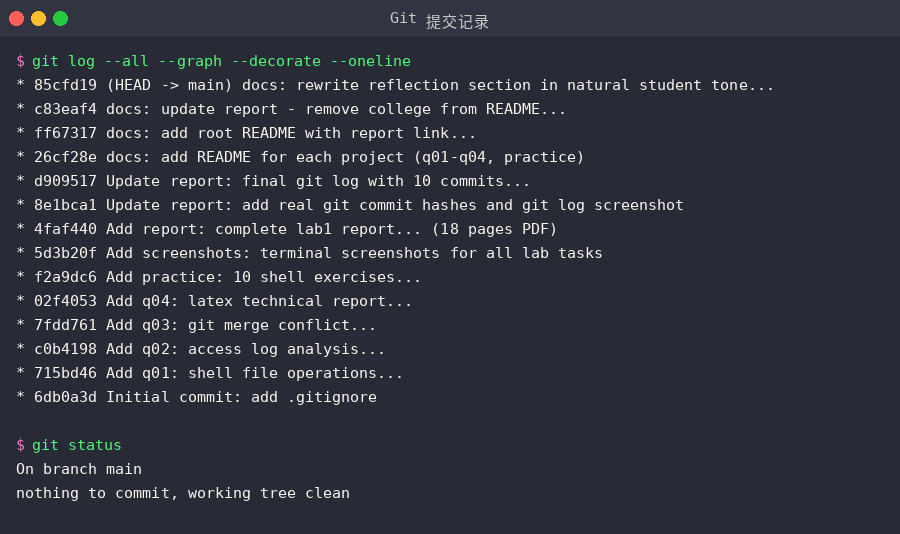
\includegraphics[width=0.9\textwidth]{git_log.png}
\caption{Git 提交历史图与工作区状态}
\label{fig:gitlog}
\end{figure}

\noindent\textbf{说明}：代码已推送到个人 GitHub 仓库：\url{https://github.com/BugMaker-orz/pc-basic-class-homework}，共完成 13 次分次提交，禁止单次全量提交。

\vspace{1cm}
\noindent\rule{\textwidth}{0.4pt}
\begin{center}
\textit{报告结束}
\end{center}

\end{document}
